\section{Causes of Inefficiencies}
\label{sec:causes}


After studying the 64 performance issues in the \numpactions problematic actions and the \numissues issues reported in the applications' bug-tracking systems, we categorize the inefficiency causes into three categories: ORM API misuses, database design, and application design. In the following we discuss these causes and how developers have addressed them. We believe these causes apply to applications built using other ORM frameworks as well, as we will discuss in Section~\ref{sec:dis}. 
%The performance causes that we have observed from performance issue tracking systems and performance action profiling are largely consistent. Also, the way how developers fix the performance issues from issue tracking systems are consistent with what we have done for the profiling issues. Consequently, we will discuss them together below. 

%\shan{are these ALL inefficiency problems or ALL inefficient-data-processing problems?}\shan{What about rendering problems; rendering template optimization?}

\begin{comment}

\end{}

\newcolumntype{g}{>{\columncolor{Gray}}r}
\begin{table*}[]
\centering
\small
\caption{Causes for problematic actions and performance issues}
\label{tab:freq}
\begin{tabular}{@{}llggggggggggggg@{}}
\toprule

\rowcolor{white}
 & Causes &Ds & Lo & Gi & Re & Sp & Ro & Fu & Tr & Da & On & FF & OS& SUM  \\
 \midrule
\rowcolor{white}
 & Inefficient  & { 0} & {0} & 0 & 0 & 0 & 1 & 0 & 1 & 2 & 2 & 2 & 0 & 8 \\
\cmidrule{3-15}
 & computation & 0 & 0 & 3 & 6 & 5 & 0 & 0 & 2 & 2 & 0 & 0 & 0 & 18 \\ 
\cmidrule{2-15}

\rowcolor{white}
 & Unnecessary  & 0 & 3 & 0 & 0 & 0 & 0 & 0 & 0 & 0 & 0 & 2 & 0 & 5 \\
\cmidrule{3-15}
API & Computation & 1 & 0 & 3 & 4 & 4 & 1 & 0 & 1 & 2 & 1 & 0 & 0 & 17 \\
\cmidrule{2-15}

\rowcolor{white}
Usage & Inefficient  & 0 & 1 & 0 & 0 & 3 & 2 & 0 & 2 & 2 & 3 & 0 & 1 & 14 \\
\cmidrule{3-15}
 &data accessing  & 3 & 0 & 4 & 5 & 10 & 0 & 0 & 2 & 0 & 2 & 0 & 0 & 26 \\
\cmidrule{2-15}
\rowcolor{white}
 & Unnecessary & 0 & 0 & 1 & 0 & 0 & 0 & 0 & 0 & 0 & 0 & 0 & 0 & 1 \\
\cmidrule{3-15}
 & data loading  & 2 & 0 & 3 & 1 & 2 & 0 & 0 & 0 & 0 & 0 & 0 & 0 & 8 \\
\cmidrule{2-15}
 \rowcolor{white}
 & Inefficient Rendering & 0 & 3 & 1 & 0 & 0 & 0 & 0 & 1 & 0 & 0 & 0 & 0 & 5 \\
\midrule


\rowcolor{white}
 & Missing  & 0 & 0 & 0 & 1 & 0 & 0 & 0 & 0 & 0 & 0 & 1 & 1 & 3 \\
\cmidrule{3-15}
 & Fields & 0 & 2 & 0 & 0 & 2 & 0 & 0 & 0 & 0 & 0 & 1 & 0 & 5 \\
\cmidrule{2-15}

\rowcolor{white}
Database& Missing  & 0 & 0 & 0 & 0 & 0 & 0 & 0 & 1 & 0 & 0 & 0 & 0 & 1 \\
\cmidrule{3-15}
 Design& association & 0 & 1 & 0 & 0 & 1 & 0 & 0 & 0 & 1 & 0 & 0 & 0 & 3 \\
 
\cmidrule{2-15}

\rowcolor{white}
   & Missing  & 0 & 1 & 0 & 0 & 0 & 0 & 0 & 0 & 0 & 0 & 2 & 0 & 3 \\
\cmidrule{3-15}
 & index & 3 & 1 & 4 & 6 & 3 & 0 & 0 & 3 & 5 & 1 & 1 & 3 & 30 \\
\midrule

\rowcolor{white}
& Unworthy  & 1 & 0 & 0 & 2 & 0 & 2 & 6 & 10 & 0 & 1 & 0 & 0 & 22 \\
\cmidrule{3-15}
App & content & 5 & 1 & 1 & 0 & 0 & 1 & 0 & 3 & 1 & 0 & 0 & 2 & 14 \\
 \cmidrule{2-15}
\rowcolor{white}
Design & Unworthy  & 0 & 2 & 0 & 0 & 0 & 0 & 0 & 0 & 0 & 0 & 0 & 0 & 2 \\
 \cmidrule{3-15}
 & features & 3 & 2 & 4 & 0 & 1 & 0 & 2 & 1 & 2 & 1 & 1 & 2 & 19 \\
 \midrule
 

\rowcolor{white}
SUM &  & 18 & 17 & 24 & 25 & 31 & 7 & 8 & 27 & 17 & 11 & 10 & 9 & 204\\
\bottomrule
\end{tabular}
\\
\footnotesize{data with white background is for problematic actions from 12 representative applications\\ data with gray background is for performance issues from 12 bug-tracking systems}
\end{table*}
\end{comment}
\definecolor{LightCyan}{rgb}{0.88,1,1}
%\definecolor{Gray}{gray}{0.9}
\definecolor{Gray}{rgb}{0.6,0.6,0.6}
\newcolumntype{g}{>{\columncolor{Gray}}r}
\begin{table}[]
\centering
\small
\caption{Inefficiency causes across 12 applications}
\label{tab:freq}
\begin{tabular}{@{\hspace{0.1in}}c@{\hspace{0.1in}}g@{\hspace{0.1in}}g@{\hspace{0.1in}}g@{\hspace{0.1in}}g@{\hspace{0.1in}}g@{\hspace{0.1in}}g@{\hspace{0.1in}}g@{\hspace{0.1in}}g@{\hspace{0.1in}}g@{\hspace{0.1in}}g@{\hspace{0.1in}}g@{\hspace{0.1in}}g@{\hspace{0.1in}}g@{\hspace{0.1in}}}
\toprule

\rowcolor{white}
   &Ds & Lo & Gi & Re & Sp & Ro & Fu & Tr & Da & On & FF & OS& Sum  \\
 \midrule
\rowcolor{white}
\multicolumn{13}{c}{\bf ORM API Misuse}\\
\midrule
\rowcolor{white}
\multirow{ 2}{*}{IC}  & { 0} & {0} & 0 & 0 & 0 & 1 & 0 & 1 & 2 & 2 & 2 & 0 & 8 \\
\cmidrule{2-14}

  & 0 & 0 & 3 & 6 & 5 & 0 & 0 & 2 & 2 & 0 & 0 & 0 & 18 \\ 
\cmidrule{1-14}

\rowcolor{white}
\multirow{ 2}{*}{UC}   & 0 & 3 & 0 & 0 & 0 & 0 & 0 & 0 & 0 & 0 & 2 & 0 & 5 \\
\cmidrule{2-14}
  & 1 & 0 & 3 & 4 & 4 & 1 & 0 & 1 & 2 & 1 & 0 & 0 & 17 \\
\cmidrule{1-14}

\rowcolor{white}
 \multirow{ 2}{*}{ID}   & 0 & 1 & 0 & 0 & 3 & 2 & 0 & 3 & 2 & 3 & 0 & 1 & 15 \\
\cmidrule{2-14}
   & 3 & 1 & 4 & 5 & 11 & 0 & 0 & 2 & 1 & 2 & 0 & 0 & 29 \\
\cmidrule{1-14}
\rowcolor{white}
  \multirow{ 2}{*}{UD}  & 0 & 0 & 1 & 0 & 0 & 0 & 0 & 0 & 0 & 0 & 0 & 0 & 1 \\
\cmidrule{2-14}
    & 2 & 0 & 3 & 1 & 2 & 0 & 0 & 0 & 0 & 0 & 0 & 0 & 8 \\
\cmidrule{1-14}
 \rowcolor{white}
   IR & 0 & 3 & 1 & 0 & 0 & 0 & 0 & 1 & 0 & 0 & 0 & 0 & 5 \\
\midrule

\rowcolor{white}
\multicolumn{13}{c}{\bf Database Design Problems}\\
\midrule
\rowcolor{white}
  \multirow{ 2}{*}{MF}   & 0 & 0 & 0 & 1 & 0 & 0 & 0 & 0 & 0 & 0 & 1 & 1 & 3 \\
\cmidrule{2-14}
   & 0 & 2 & 0 & 0 & 2 & 0 & 0 & 0 & 0 & 0 & 1 & 0 & 5 \\
\cmidrule{1-14}
\rowcolor{white}
   \multirow{ 2}{*}{MI}   & 0 & 1 & 0 & 0 & 0 & 0 & 0 & 0 & 0 & 0 & 2 & 0 & 3 \\
\cmidrule{2-14}
   & 3 & 1 & 4 & 6 & 3 & 0 & 0 & 3 & 5 & 1 & 1 & 3 & 30 \\
\midrule
\rowcolor{white}
\multicolumn{13}{c}{\bf Application Design Tradeoffs}\\
\midrule
\rowcolor{white}
 \multirow{ 2}{*}{DT}   & 1 & 0 & 0 & 2 & 0 & 2 & 6 & 10 & 0 & 1 & 0 & 0 & 22 \\
\cmidrule{2-14}
  & 5 & 1 & 1 & 0 & 0 & 1 & 0 & 3 & 1 & 0 & 0 & 2 & 14 \\
 \cmidrule{1-14}
\rowcolor{white}
  \multirow{ 2}{*}{FT}   & 0 & 2 & 0 & 0 & 0 & 0 & 0 & 0 & 0 & 0 & 0 & 0 & 2 \\
 \cmidrule{2-14}
  & 3 & 2 & 4 & 0 & 1 & 0 & 2 & 1 & 2 & 1 & 1 & 2 & 19 \\
 \midrule
 

\rowcolor{white}
Sum  & 18 & 17 & 24 & 25 & 31 & 7 & 8 & 27 & 17 & 11 & 10 & 9 & 204\\
\bottomrule
\end{tabular}
\\
\footnotesize{Data with white background shows 64 issues from 40 problematic actions\\ Data with gray background shows 140 issues from 12 bug-tracking systems\\
\begin{tabular}{rlrl}
IC:& Inefficient Computation & MF:& Missing Fields \\
UC:& Unnecessary Computation & MI:& Missing Indexes \\
ID:& Inefficient Data Accessing & DT:& Content Display Trade-offs\\
UD:& Unnecessary Data Retrieval & FT:& Functionality Trade-offs\\
IR:& Inefficient Rendering & \\

\end{tabular}
}

\vspace{-0.10in}
\end{table}

\subsection{ORM API Misuses} 
\label{causes:api}

About half of the performance issues that we studied suffer from API misuses. In these cases, performance can be improved by changing how the Rails APIs are used without modifying program semantics or database design. While some of these misuses appear simple, making the correct decision requires deep expertise in the implementation of the ORM APIs and query processing.

%\shan{TODO: 1.discuss scalability problems 2. add some profiling examples, instead of all examples from bug-tracking system?}
\vspace{-0.1in}

\subsubsection{Inefficient Computation (IC)}
\label{sec:inefficomp}

In these cases, the poorly performing code conducts useful computation but inefficiently.
Such cases comprise more than 10\% of the performance issues in both bug reports and problematic actions. 
\vspace{-0.18in} 
\paragraph{\bf{Inefficient queries}}
The same operation on persistent data can be implemented via different ORM calls. However, the performance of the generated queries can be drastically different. This problem has not been well studied before for ORM applications.
%A functionality can be accomplished by different database queries and developers unfortunately use a more expensive query. This problem is widespread and is difficult to avoid for developers who cannot easily track which queries are transparently generated by ORM or whether the queries are efficient. Unfortunately, there was no automated solution yet.

Figure~\ref{fig:spreeAnyVsExists} shows two ways that an online shopping system checks if there are product \texttt{variants} whose inventory are not tracked.
%(i.e., \texttt{track\_inventory} field is \texttt{false}).
The Ruby code differs only in the use of 
\texttt{any?} vs \texttt{exists?}. However, the performance of the generated queries differs substantially:
the generated query in Figure~\ref{fig:spreeAny} scans all records in the \texttt{variants} table to compute the count if no index exists, but that in Figure~\ref{fig:spreeExists} only needs to scan and locate the first 
\texttt{variant} record where the predicate evaluates to true. \texttt{Spree} developers discovered and fixed this problem in 
\texttt{Spree-6720}.\footnote{We use \texttt{A-n} to denote report number {\tt n} in application {\tt A}'s bug-tracking system.}
% we mention that this is widespread in 2 sentences
%This problem is widespread as we find that it contributes to 3 problematic actions in 2 applications. 
Our profiling finds similar problems. For example, simply replacing \texttt{any?} with \texttt{exists?} in a problematic action of \texttt{OneBody} improves server time by 1.7$\times$. 
%\alvin{how about say how much improvement for the spree code shown rather than citing another example?}
Our static checker that will be discussed in Section~\ref{sec:dis} finds that this is a common problem as it appears in the latest versions of 9 out of 12 applications under study.

\begin{comment}
\begin{figure}[h]
  \centering
  \begin{subfigure}[t]{0.5\textwidth}
  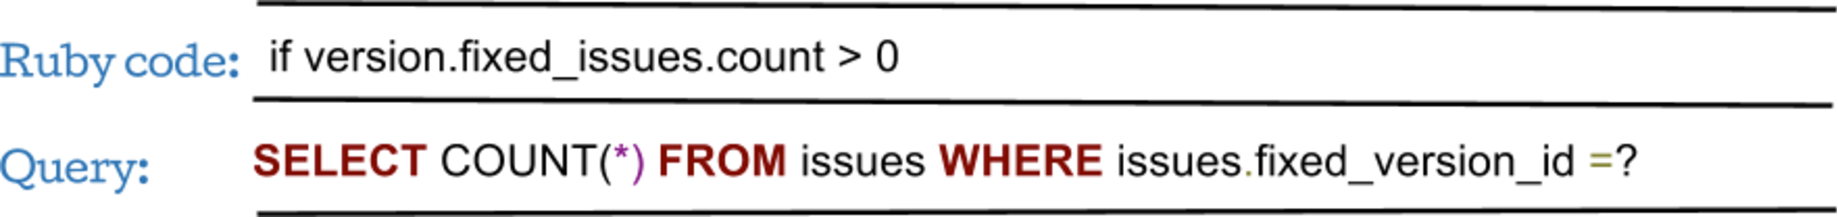
\includegraphics[width=0.95\columnwidth]{figs/countstar}
  %\caption{Inefficient API}
  \label{InefficientAPI}
  \end{subfigure}
  
    \centering
  \begin{subfigure}[t]{0.5\textwidth}
  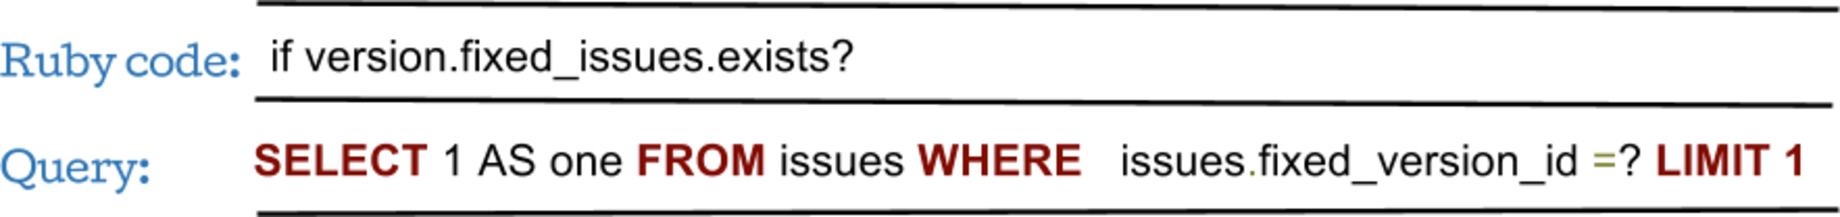
\includegraphics[width=0.95\columnwidth]{figs/exist}
  	%\caption{Efficient API}
  \label{efficientAPI}
  \end{subfigure}

  \caption{Inefficient query due to improper APIs in Redmine}
  \label{API}
\end{figure}
\end{comment}

\begin{comment}
\begin{figure}[h]
  \centering
  \begin{subfigure}
      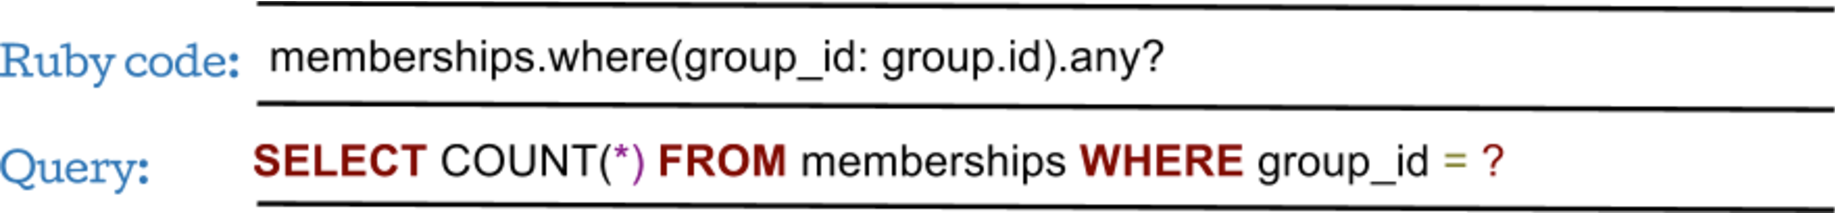
\includegraphics[width=0.95\columnwidth]{figs/any}
      \caption{Inefficient API}
      
      \label{fig:any}
  \end{subfigure}
  
  \begin{subfigure}
    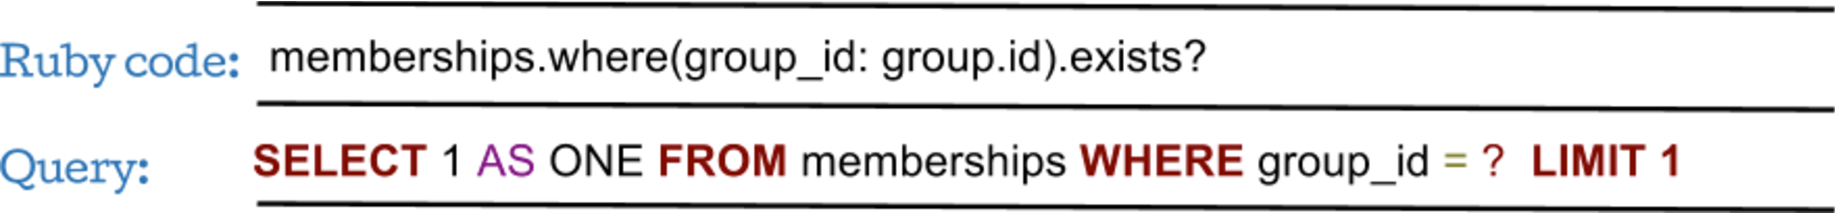
\includegraphics[width=0.95\columnwidth]{figs/exists}
  	\caption{Efficient API}
    \label{fig:exists}
  \end{subfigure}

  \caption{Inefficient query due to improper APIs in Onebody}
  \label{fig:anyVsExists}
\end{figure}
\end{comment}

% \begin{figure}
% \centering
% \label{fig:sl}
%     \begin{subfigure}
%     \centering
%         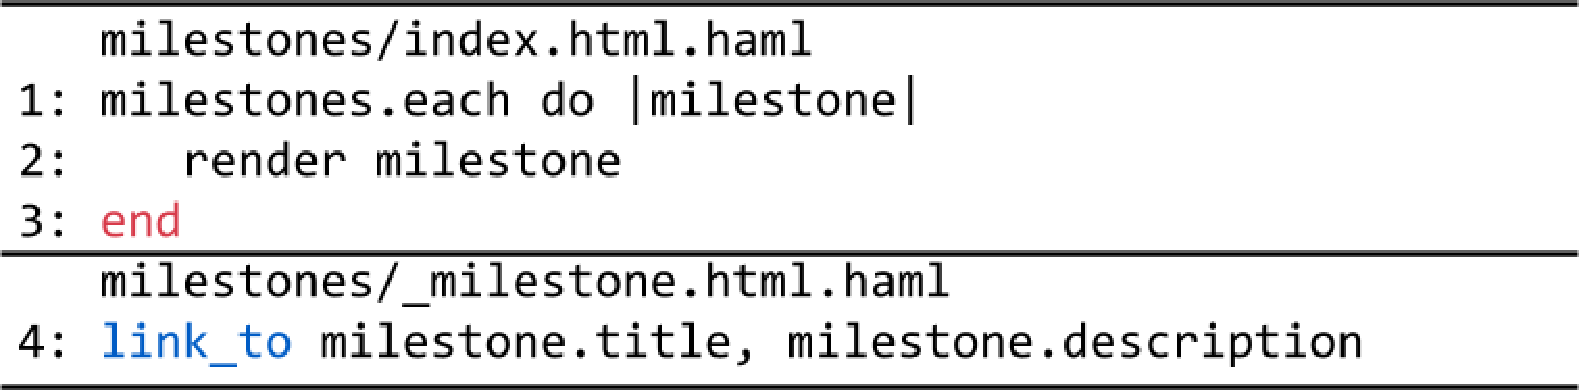
\includegraphics[width=0.4\linewidth]{hownotto/partialA.pdf}
%       \caption{Inefficient partial rendering}
%          \label{fig:partialA}
%     \end{subfigure}
%     \begin{subfigure}
%         \centering
%         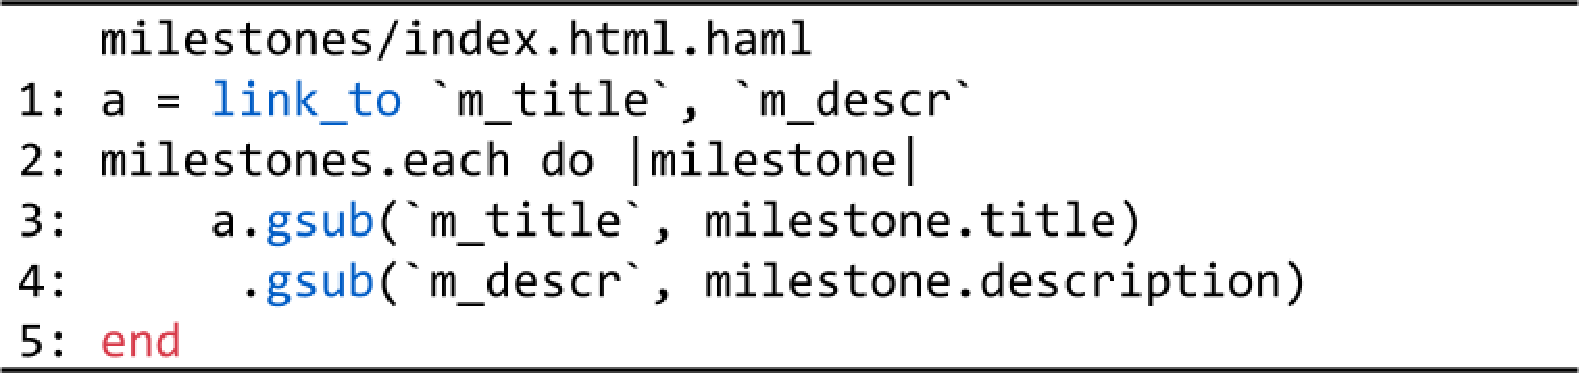
\includegraphics[width=0.4\linewidth]{hownotto/partialB.pdf}
%       \caption{Efficient partial rendering}
%         \label{fig:partialB} 
%     \end{subfigure}
% \caption{Inefficient partial rendering in Gitlab}
% \end{figure}

\begin{figure}
  \centering
  \begin{subfigure}
    \centering
    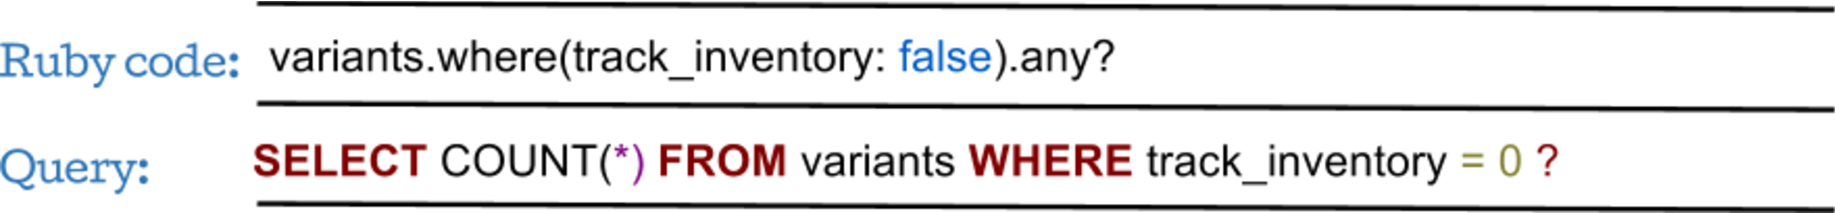
\includegraphics[width=0.5\columnwidth]{figs/spreeAny}
    \caption{Inefficient}
    \label{fig:spreeAny}
  \end{subfigure}
  
  \begin{subfigure}
      \centering
      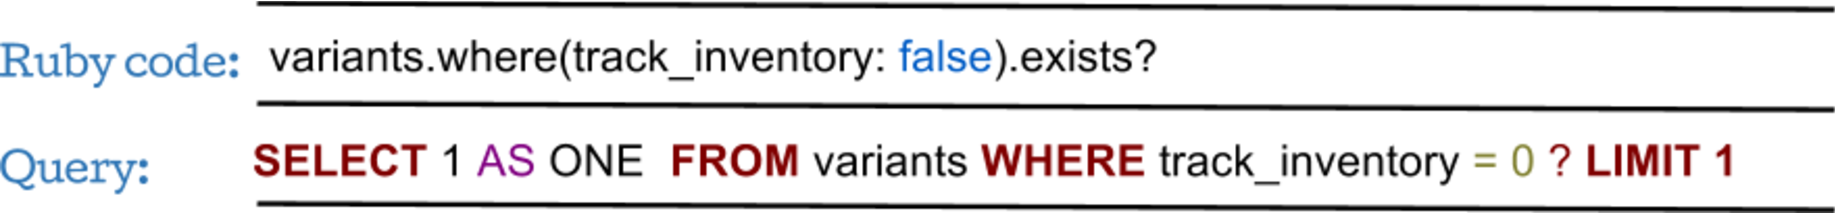
\includegraphics[width=0.5\columnwidth]{figs/spreeExists}
      \caption{Efficient}
      \label{fig:spreeExists}
  \end{subfigure}
  \caption{Different APIs cause huge performance difference}
  %Inefficient query due to improper APIs in Spree}
  \label{fig:spreeAnyVsExists}
\end{figure}

Another common problem is developers using API calls that generate queries with unnecessary ordering of the results. For example, Ror, Diaspora, and Spree developers use \texttt{Object.}\texttt{where(c).first} to get an object satisfying predicate \texttt{c} instead of \texttt{Object.find\_by(c)}, not realizing that the former API orders {\tt Object}s by primary key after evaluating predicate {\tt c}. 
As a fix, both Gitlab and Tracks developers explicitly add \texttt{except(:order)} in 
the patches to eliminate unnecessary ordering in the queries, further showing how simple changes can lead to drastic performance difference.

\vspace{-0.08in} 
\paragraph{\bf{Moving computation to the DBMS}} %Should Be a Query}}
As the ORM framework hides the details of query generation, developers often write code that results in multiple queries being generated. Doing so incurs extra network round-trips, or running computation on the server rather than the DBMS, which leads to performance inefficiencies.

%
%A functionality is faster to accomplish by one query. Unfortunately, the developers use either (1) multiple queries or (2) one query together with in-memory computation. Either way, inefficiency is incurred by extra query and/or data round-trips. Although the general problem of pushing application computation down to database has been tackled by previous work \cite{cheung:pldi13} using program synthesis, our study finds that many such problems in Rails are caused by simple API misuses and hence could benefit from a new tool that is less general but much simpler.
%
%There are many cases that only involve one expression and simple API misuses.
For example, the patch of \texttt{Spree-6720} replaces
\texttt{if(exist?)} \texttt{find; else create} with 
\texttt{find\_or\_create\_by}, where the latter combines two queries that are issued by \texttt{exist}
and \texttt{find}/\texttt{create} into one.
The patch of \texttt{Spree-6950} replaces
\texttt{pluck(:total).sum} with \texttt{sum(:total)}. The former uses \texttt{pluck} to issue
a query to load the \texttt{total} column of all corresponding records and then
computes the sum in memory, while the latter uses \texttt{sum} to issue a 
query that directly performs the sum in the DBMS without returning actual records to the server.
The patch of {\tt Gitlab-3325} replaces \texttt{pluck(:id)+pluck(:id)}, which replaces two queries and an in-memory union via {\tt +} with one SQL \texttt{UNION} query, in effect 
moving the computation to the DBMS.
%conducts the summation in database and hence saves data loading time. 
%This was from the bug-tracking system of Gitlab, and we also see similar cases in Spree.
Such API misuses are very common and occur in many applications as we 
will discuss in Section~\ref{sec:dis}. 



%For example, xxx developers use \texttt{array.count} instead of \texttt{array.size} to get the size of an array. When \texttt{array} is already loaded in memory, the former issues a query to do the counting in database, while the latter conducts in-memory size computation and hence is much more efficient.

There are also more complicated cases where a loop implemented in Ruby can be completely pushed
down to DBMS,  which has been addressed in
previous work using program synthesis~\cite{cheung:pldi13}.

%where the Rails program iterate through a container
%filled with data previously loaded from database 
%As another example, it could cause many rows to be loaded to memory for selection that should have been done in database.
%An example of row-wise unnecessary data retrieval is shown in Fig \ref{rowwise}. Ruby code in Fig \ref{posts} from \texttt{Spree-6903} first retrieves all posts of ``StatusMessage'' type, and then through \texttt{tagged\_with}, only posts with specified \texttt{tagged\_name} will be rendered. Other posts are useless. A better way to avoid unnecessary data is to issue another query which will only retrieve the posts with specified \texttt{tag\_name} as shown in Fig \ref{taggings}. This simple change would save the corresponding action in software xxx xx based on our profiling.

%Redundant row retrieval problem has not been studied by previous work.
%\shan{is this right?} 

%Furthermore, it is difficult for developers to avoid this problem. In fact, the more efficient code shown in Figure \ref{rowwise} may actually be considered as ``message chain'' code smell. It is difficult for developers to realize that such smell code is actually much more efficient. Future work should build xx to automatically detect and fix this xxx.

%\begin{figure}[h]
%  \centering
%  \begin{subfigure}[t]{0.5\textwidth}
%  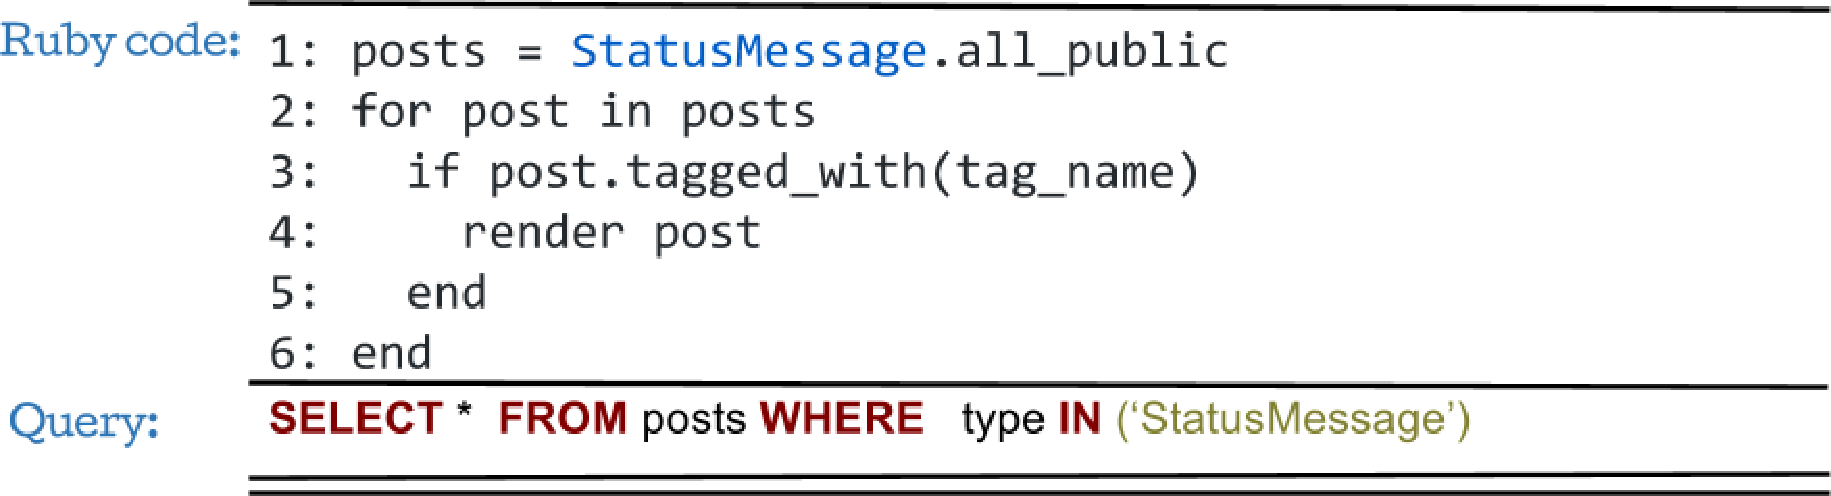
\includegraphics[width=1\columnwidth]{figs/posts}
%  \caption{Unoptimized} 
%  \label{posts}
%  \end{subfigure} 
%    \centering
%  \begin{subfigure}[t]{0.5\textwidth}
%  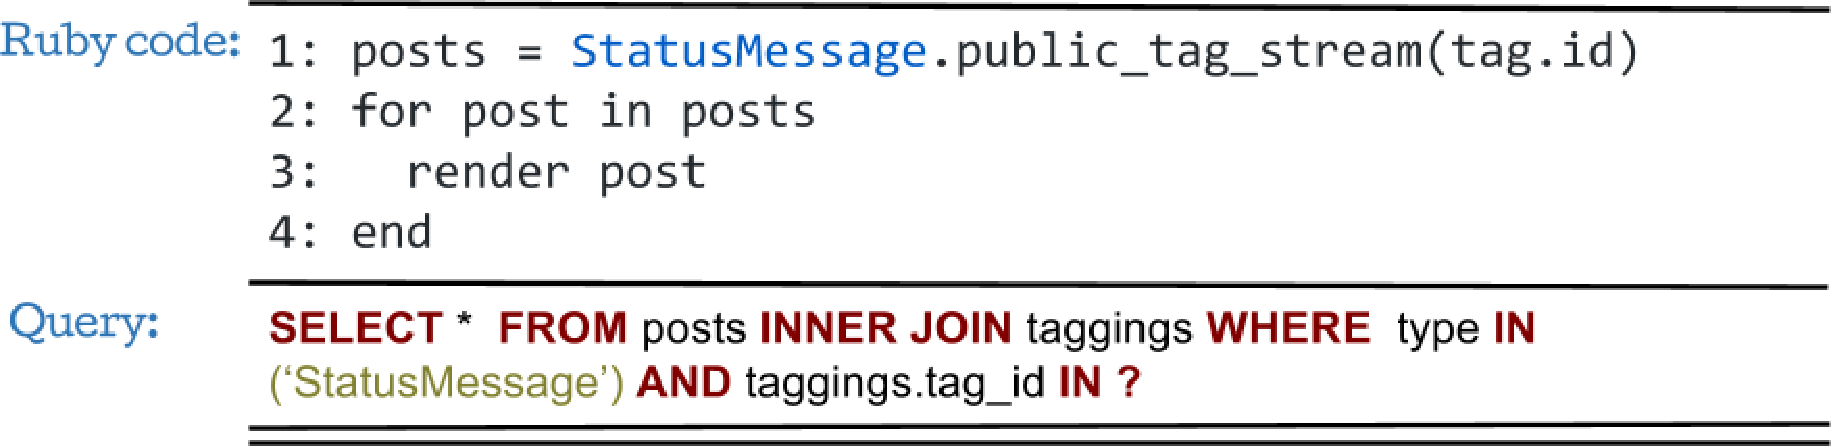
\includegraphics[width=1\columnwidth]{figs/taggings}
%  	\caption{Optimized}
%  \label{taggings}
%  \end{subfigure}
%  \caption{Unnecessary row-data retrieval in xxx}
%  \label{rowwise}
%\end{figure}
\vspace{-0.08in} 
\paragraph{\bf{Moving computation to the server}} %Should Not be a Query}} 
Interestingly, there are cases where the computation should be moved to the server from the DBMS. %a functionality is faster to do by in-memory computation instead of a database query. 
As far as we know, this issue has not been studied before. 
%and is naturally out of the scope of database optimization. 

%
For example, in the patch of \texttt{Spree-6819}, developers replace 
\texttt{Objects.count} with \texttt{Objects.size} in 17 different locations, as
\texttt{count} always issues a \texttt{COUNT} query while \texttt{size} counts the 
\texttt{Objects} in memory
if they have already been retrieved from the database by earlier computation.
%and issues a count SQL query otherwise. 
%However, as all instances are in views (not controllers) or in utility functions, merging them with other code such that the appropriate call can be made will break code modularity, making it a difficult choice for developers.
%Consequently, code modularity concerns prevent them from being merged with other queries. 
Such issues are also reported in {\tt Gitlab-17960}.

\vspace{-0.08in} 
\paragraph{\bf{Summary}} Rails, like other ORM frameworks, lets developers implement a given functionality in various ways.
%With ORM framework, a functionality can often be implemented by different combinations of queries and in-memory computation. 
Unfortunately, developers often struggle at 
picking the most efficient option. The deceptive names of many 
Rails APIs like \texttt{count} and \texttt{size} make this even more challenging. Yet, we believe many cases can be fixed using simple static analyzers, as we will discuss in Section~\ref{sec:dis}.
%Meanwhile, many inefficient API patterns are simple and repeatedly appear in different applications. It is both feasible and very helpful to build static analysis tools to automatically identify and/or fix inefficient API uses. More complicated cases would benefit from general query synthesis techniques \cite{cheung:pldi13}.

\begin{figure}
  \centering
  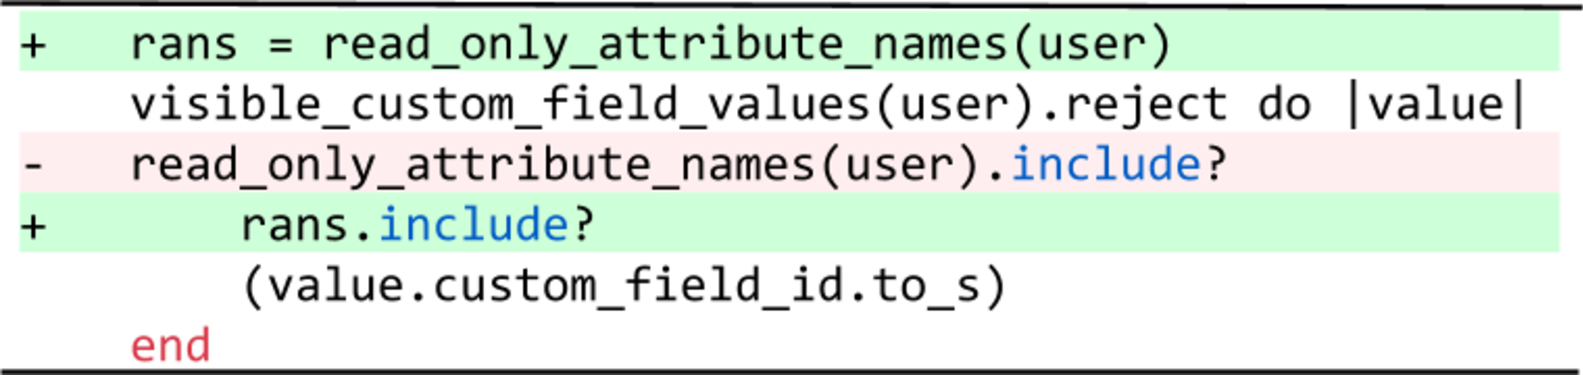
\includegraphics[width=0.7\columnwidth]{hownotto/redCom}
  \caption{A loop-invariant query in Redmine}
  \label{fig:redCom}
\end{figure}

\subsubsection{Unnecessary Computation (UC)} 
\label{sec:uncomp}
More than 10\% of the performance issues are caused by (mis)using ORM APIs that lead to unnecessary queries being issued. This type of problems has not been studied before.
%The poorly performing code issues unnecessary queries. It happens for about 10\% of studied performance issues, and also causes problematic actions in the latest versions of multiple applications.
\vspace{-0.08in} 
\paragraph{\bf{Loop-invariant queries}}
Sometimes, queries are repeatedly issued to load the {\it same} database contents and hence are unnecessary. 
%In traditional programs, these problems can be solved by classic optimization techniques, which we will discuss below. Unfortunately, problems here require the optimizer to understand both ORM/query semantics and Ruby application semantics, and have not been tackled by previous research.
%
%Sometimes, a query is repeatedly issued in a loop to return the same content --- it could be optimized by \textit{loop-invariant code motion} if the optimizer understands not only Ruby logic but also ORM and queries.
For instance, Figure~\ref{fig:redCom} shows the patch from \texttt{redmine-23334}.
This code iterates through every custom field 
\texttt{value} %that is visible to the \texttt{user} 
and retains only those that 
\texttt{user} has write access to.
%, \texttt{reject}ing the read-only ones. 
To conduct this access-permission checking, in every iteration, \texttt{read\_only\_attribute\_}
\texttt{names(user)} issues a query to get the names of all read-only fields of \texttt{user}, as shown by the red highlighted line
in the figure. Then, if
\texttt{value} belongs to this read-only set, it will be excluded from the return set of this function (i.e., the \texttt{reject} at the beginning of the loop takes effect). Here, the \texttt{read\_only\_attribute\_names(user)} query 
returns exactly the same result during every iteration of the loop and causes
unnecessary slowdowns. 
%\alvin{I am confused. What is the original code? The red line? Why are we showing the a patch but not discussing it. Add line numbers?}
As shown by the green lines in figure, Redmine developers hoist loop invariant \texttt{read\_only\_attribute\_names(user)} outside the loop and achieve more than 20$\times$ speedup for the corresponding function for their workload.
%, shortening its time from 1.03 second to 0.05 second with 1000 issues.
Similar issues also occur in Spree and Discourse.





\vspace{-0.08in} 
\paragraph{\bf{Dead-store queries}}
In such cases, queries are repeatedly issued to load {\it different} database contents into the same memory object while the object has not been used between the reloads.
%without using the object in between --- it could be optimized by
%\textit{dead-store elimination} if the optimizer understands not only Ruby but also ORM and queries. 
 For example, in Spree, every shopping transaction has a corresponding
 {\tt order} record in the {\tt orders} table. This table has a
 {\tt has\_many} association relationship with the 
 {\tt line\_items} table, meaning that every order  contains
 multiple lines of items. Whenever the user updates his/her shopping
 cart, the {\tt line\_items} table would change, at which point the old version of Spree always uses an {\tt order.reload} to make 
 sure that the in-memory copy of {\tt order} and its associated 
 {\tt line\_item}s are up-to-date. Later on, developers realize that
 this repeated reload is unnecessary, because the content of 
 {\tt order} is not used by the program until check out.
 Consequently, in {\tt Spree-6379}, developers remove many 
 {\tt order.reload} from model classes, and instead add it in a few places in the {\tt before\_payment} action of the
 {\tt checkout} controller, where the {\tt order} object is to be used.
%\alvin{how does this justify issuing repeated reads?} 


%original listing
\begin{comment}

\begin{lstlisting}[language=Ruby, numbers=left, firstnumber=1, numberstyle=\tiny\color{gray}, caption={redundant computation from redmine~\cite{redmine}.},label={redundantComputation}, numbers = none]
@\lstlabel{redundantComputation}@ visible_custom_field_values(user).reject do |value| 
 read_only_attribute_names(user).include?(value.custom_field_id.to_s) 
@\lstlabel{end}@ end
\end{lstlisting}

\begin{lstlisting}[language=Ruby, numbers=left, firstnumber=1, numberstyle=\tiny\color{gray}, caption={remove redundant computation from redmine~\cite{redmine}.},label={removeredundantComputation}, numbers = none]
@\lstlabel{removeredundantComputation}@ 
read_only_attr_names_array = read_only_attribute_names(user)
visible_custom_field_values(user).reject do |value|
  read_only_attr_names_array.include?(value.custom_field_id.to_s)
end
\end{lstlisting}

\end{comment}

\begin{figure}

  \centering
  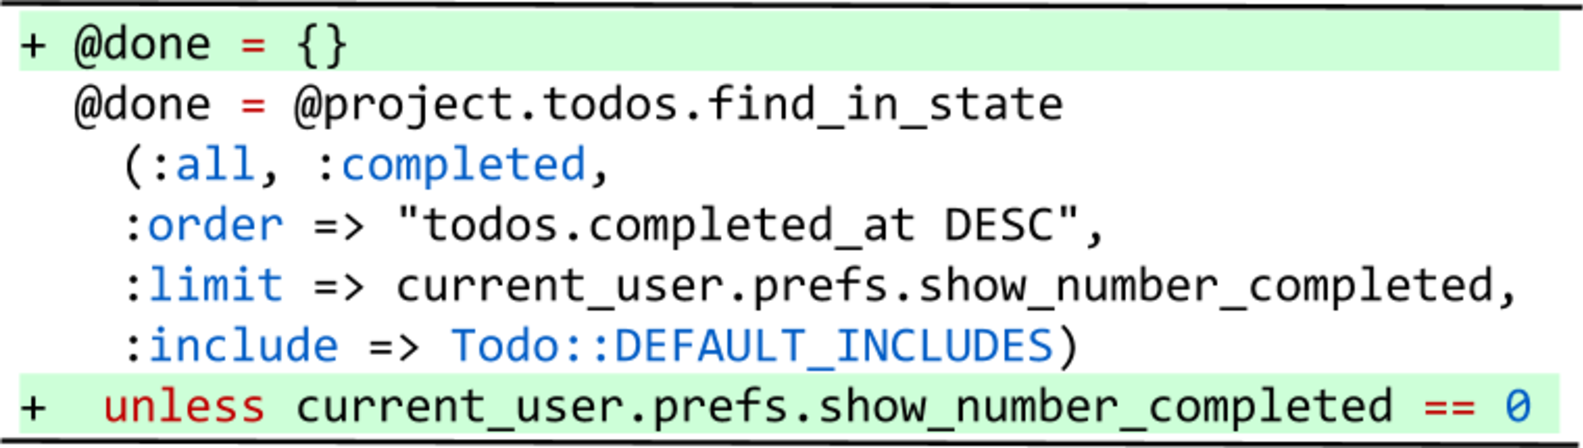
\includegraphics[width=0.7\columnwidth]{hownotto/tracks63}
  \caption{A query with known results in Tracks}
  \label{fig:tracks63}
\end{figure}

\vspace{-0.08in} 
\paragraph{\bf{Queries with known results}}
A number of issues are due to issuing queries whose results are already known, hence incurring unnecessary network round trips and query processing time.
%Occasionally, certain value of a Rails API parameter would cause the corresponding query to return a predictable constant result. If that specific parameter value is common, it is better to issue the query conditionally. This optimization again requires knowledge about both application semantics and ORM/query, and is not handled by existing techniques.
%
An example is in \texttt{Tracks-63}. As shown in Figure~\ref{fig:tracks63},
the code originally issues a query to retrieve up to 
\texttt{show\_number\_completed} number of completed tasks. Clearly, when \texttt{show\_number\_completed} is $0$, the query always returns an empty set due to {\tt limit} being $0$.
Developers later realize
that $0$ is a very common setting for \texttt{show\_number\_completed}. 
%In fact, the corresponding view file \texttt{show.html.erb} has already been designed to render the completed-todo panel only conditionally.
Consequently, they applied the patch shown in Figure \ref{fig:tracks63} to only issue the query when needed. 
%\alvin{say something about how prevalent this is?}

\vspace{-0.08in} 
\paragraph{\bf{Summary}}
While similar issues in general purpose programs can be eliminated using classic compiler optimization techniques (e.g., loop invariant motion, dead-store elimination), doing so for ORM applications is difficult as it involves understanding database queries.
% and performing inter-action data-flow analysis. 
We are unaware of any compilers that perform such transformations.
%Correctly detecting and fixing unnecessary computation discussed above are non-trivial. 
%Furthermore, they often require inter-action data-flow analysis. 
%ORM developers will benefit from techniques that integrate ORM and database knowledge into traditional compiler optimization techniques like loop-invariant code motion, dead-store elimination, and others.

\vspace{-0.08in} 
\subsubsection{Inefficient Data Accessing (ID)} 
\label{sec:iffidata}
Problems under this category suffer from data transfer slow downs, including not batching data transfers (e.g., the well-known ``N+1'' problem) or batching too much data into one transfer.

\vspace{-0.08in} 
\paragraph{\bf{Inefficient lazy loading}}
As discussed in Section~\ref{sec:background}, when a set of objects $O$ in table $T_1$ are requested, objects stored in table $T_2$ associated with $T_1$ and $O$ can be loaded together through eager loading. If lazy loading is chosen instead, 
one query will be issued to load $N$ objects from $T_1$, and then
$N$ separate queries have to be issued to load associations of each such object from $T_2$. This is known as the ``N+1'' query problem. While prior work has studied this problem~\cite{nplusone, cheung:sigmod14:sloth, bullet}, we find it still prevalent: it appears in 15 problematic actions and 9 performance issues in our study. 
%This is a well known problem and can be tackled by research techniques \cite{} and Rails plugins \cite{bullet}.

Figure~\ref{fig:nplusone} shows an example that we find in the latest version of Lobsters, where the deleted code retrieves 50 \texttt{mods} objects. Then, for each \texttt{mod}, a query is issued to retrieve its associated \texttt{story}. Using eager loading in the added line, all 51 queries (and hence 51 network round-trips) will be combined together. In our experiments, the optimization reduces the end-to-end loading time of the corresponding page from 1.10 seconds to 0.34 seconds.

% Bullet is a rails gem, Sloth
%Several previous work can help developers avoid the above lazy loading problems. For example, a Rails plugin, Bullet\cite{bullet}, can warn developers about ``N + 1'' problems and remind them to use eager loading. Sloth \cite{cheung:sigmod14:sloth} will automatically batch queries to avoid N + 1 queries without developers' specifying loading strategies
%\shan{hmm, is this lazy loading or eager loading}.


\begin{figure}
  \centering
  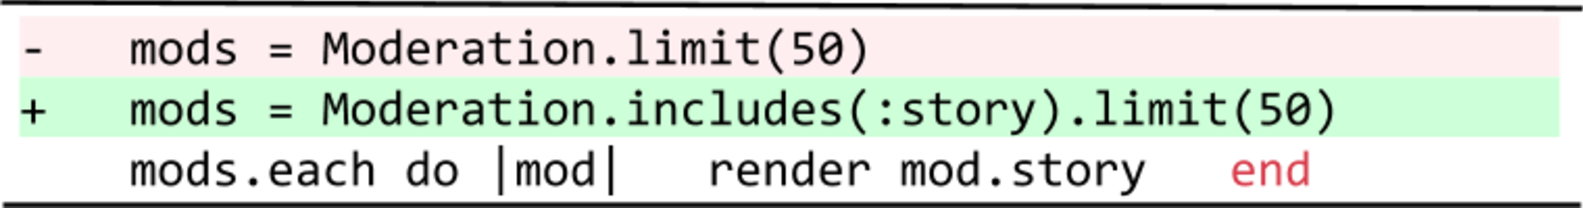
\includegraphics[width=0.7\columnwidth]{hownotto/moderations}
  \caption{Inefficient lazy loading in Lobsters}
  \label{fig:nplusone}
\end{figure}

\begin{comment}
\begin{lstlisting}[language=Ruby, numbers=left, firstnumber=1, numberstyle=\tiny\color{gray}, caption={N + 1 queries from redmine~\cite{redmine}.},label={nplusone}]
mods = Moderation.order("id desc").limit(50)
mods.each do |mod|
  if mod.user
  	puts mod.user.username
  end
end
\end{lstlisting}

\begin{lstlisting}[language=Ruby, numbers=left, firstnumber=1, numberstyle=\tiny\color{gray}, caption={remove N + 1 queries from lobsters~\cite{lobsters}\shan{redmine?}.},label={rmnplusone}, numbers = none]
mods = Moderation.includes(:user).order("id desc").limit(50)
\end{lstlisting}
\end{comment}

\vspace{-0.08in} 
\paragraph{\bf{Inefficient eager loading}}
However, always loading data eagerly can also cause problems. \textcolor{black}{ Specifically, when the associated objects are too large, loading them all at once will create huge memory pressure and even make the application unresponsive.}
In contrast to the ``N+1'' lazy loading problem, there is little support for developers to detect eager loading problems. %\junwen{it seems in the profiling result all about inefficient lazy loading}

In \texttt{Spree-5063}, a Spree user complains that their installation performs very poorly on the product search page. Developers found that the problem was due to eager loading shown in Figure~\ref{fig:spree5063}.
In the user's workload, while loading 405 \texttt{products} to display on the page, eager loading causes 13811 related \texttt{variants} products containing 276220 \texttt{option\_values} (i.e., product information data) to be
loaded altogether, making the page freeze. As shown in 
Figure \ref{fig:spree5063}, the patch delays the loading of
\texttt{option\_values} fields of \texttt{variants} products. Note that these
\texttt{option\_values} are needed by later computation, and the patch
delays but not eliminates their loading.

\begin{figure}
  \centering
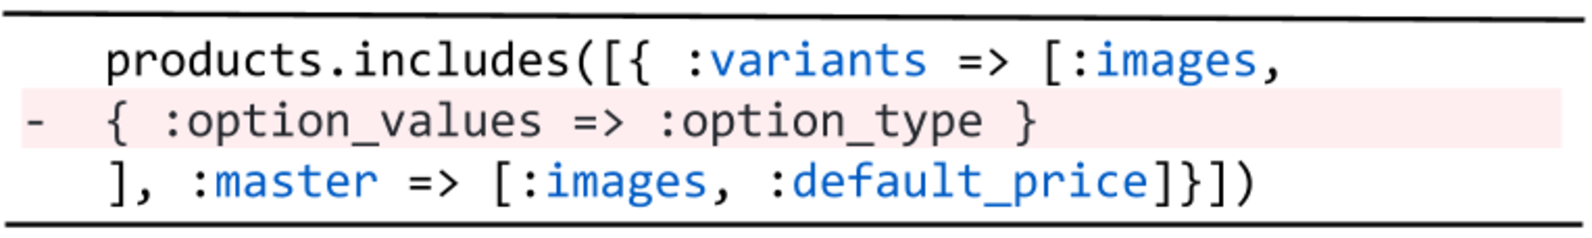
\includegraphics[width=0.7\columnwidth]{hownotto/spree5063}
  \caption{Inefficient eager loading in Spree}
  \label{fig:spree5063}
  \vspace{-0.25in}
\end{figure}

%When loadING a \texttt{product}, the corresponding \texttt{variants} and its \texttt{option\_values} and \texttt{option\_types} will be retrieved together. It is complained that it can cause the ruby process to lock up on large data sets (405 \texttt{products}/13811 \texttt{variants}/48 \texttt{optoin\_types}/948 \texttt{option\_values}). Since a variant can have many \texttt{option\_values}, the variant on average could have 20 \texttt{option\_values}. In total, there could be 276220 \texttt{option\_values} to load.  %Furthermore, ``eager loading'' may retrieve data which will never be used by the application,
%\shan{is it true?}.
%\cong{N+1 is a well-known problem. I think we may need to go deeper into the cause. As for lazy loading, why would developers load more data than needed? (programmability or modularity?)} 

\vspace{-0.08in} 
\paragraph{\bf{Inefficient updating}}
Like the ``N+1'' problem, developers would issue N queries to update N records separately (e.g., \texttt{objects.each |o| o.update end}) rather than merging them into one update (e.g., \texttt{objects.update\_all}). This is reported in Redmine and Spree, and our static checker (to be discussed in Section~\ref{sec:dis}) finds this to be common in the latest versions of 6 out of the 12 studied applications. 
\vspace{-0.22in} 
\subsubsection{Unnecessary Data Retrieval (UD)} 
%Since ORM frameworks are not aware of the high level application semantics. They cannot figure out how developers will use the data returned from the DBMS. Thus,  providing optimal data retrieval approach is not an easy job.
Unnecessary data retrieval happens when software retrieves persistent data that is not used later. Prior work has identified this problem in applications built using both Hibernate~\cite{chen:se16:redundantData} and Rails~\cite{yan:cikm17}. In our study, we find this continues to be a problem in one problematic action in the latest version of Gitlab and 9 performance issue reports.
Particularly, fixing the unnecessary data retrieval in the latest 
version of Gitlab can drop the end-to-end loading time of its 
\texttt{Dashboard/Milestones/index} page from 3.0 to 1.1 seconds in our experiments.
We also see some unnecessary data retrieval caused by simple misuses
of APIs that have similar names --- \texttt{map(\&:id)} retrieves the whole
record and then returns the \texttt{id} field, yet \texttt{pluck(:id)} only
retrieves the \texttt{id} field. 
%TODO \alvin{This is a weak point given (our own) prior work and also we are not showing code. I suggest removing it if we need space.}
%there are 2 cases caused by map vs pluck
\vspace{-0.08in} 
\subsubsection{Inefficient Rendering (IR)}
\label{sec:iffirender}
IR reflects a trade-off between readability and performance when a view file renders a set of objects. It has not been studied before.

Given a list of objects to render, developers often 
%implement a function, or use an existing library function
use a library function, like \texttt{link\_to} on Line 4 of Figure~\ref{fig:partialA},
to render one object and encapsulate it in a partial view file
such as \texttt{\_milestone.html.haml} in Figure~\ref{fig:partialA}.
Then, the main view file \texttt{index.html.haml} simply applies the
partial view file repeatedly to render all objects. 
The inefficiency is that a rendering function like \texttt{link\_to}
is repeatedly invoked to generate very similar HTML code. Instead,
the view file could generate the HTML code for one object,
and then use simple string substitution, 
such as \texttt{gsub} in Figure~\ref{fig:partialB}, to quickly 
generate the HTML code for the remaining objects, avoiding redundant
computation. The latter way of
rendering degrades code readability, but improves performance substantially
when there are many objects to render or with complex rendering functions.

Although slow rendering is complained, such transformation has not yet been proposed by issue reports. Our profiling finds such optimization speeds up 5 problematic actions by 2.5$\times$ on average.
%This type of problems does not exist in the 140 issue reports that we studied. 
%However, our profiling finds the above transformation to speed up 5 problematic actions by 2.5$\times$ on average. 

\begin{figure}
\centering
\label{fig:sl}
    \begin{subfigure}
    \centering
        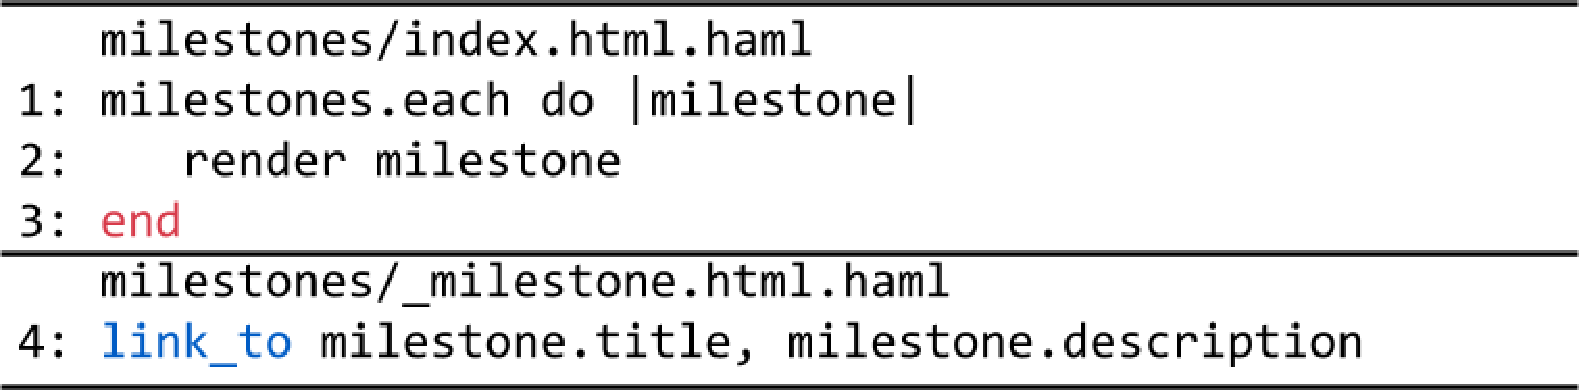
\includegraphics[width=0.4\linewidth]{hownotto/partialA.pdf}
       \caption{Inefficient partial rendering}
         \label{fig:partialA}
    \end{subfigure}
    \begin{subfigure}
        \centering
        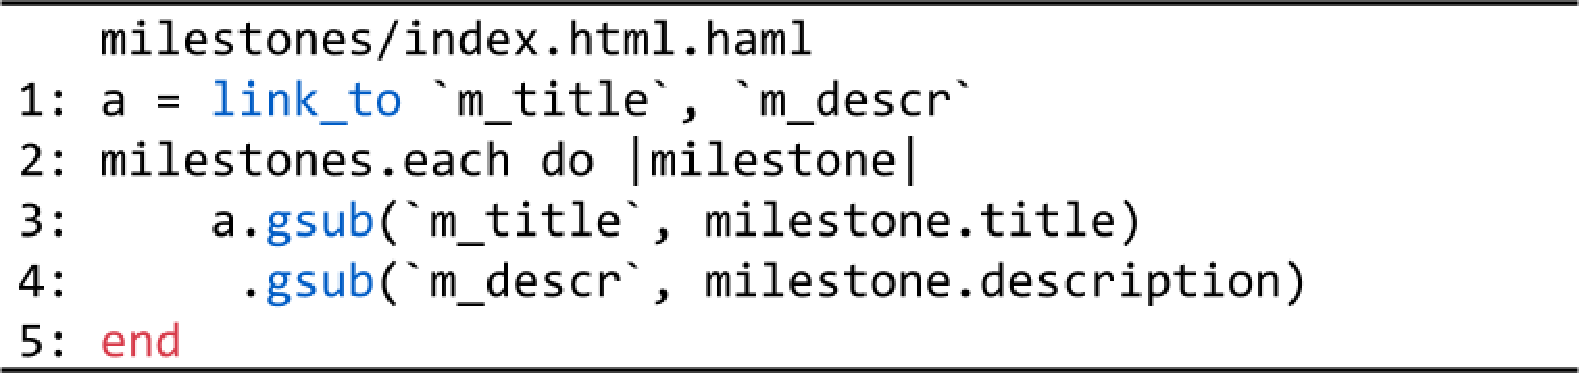
\includegraphics[width=0.4\linewidth]{hownotto/partialB.pdf}
       \caption{Efficient partial rendering}
        \label{fig:partialB} 
    \end{subfigure}
\caption{Inefficient partial rendering in Gitlab}
\end{figure}

\subsection{Database Design Problems}
\label{causes:db}

Another important cause of performance problems is suboptimal database design. Fixing it requires changing the database schema.
%Sometimes, the root cause of a performance problem is about database table design. Consequently, fixing these problems requires modifying schema and model files in ORM applications.
\vspace{-0.08in} 
\subsubsection{Missing Fields (MF)}
\label{sec:addfield}
%ORM frameworks encourage developers to maintain all classes to be stored in the database as model classes \alvin{what does Rails call such classes?} \alvin{find something to cite if possible regarding standard practices} for modularity and code maintenance. 
Deciding which object field to be physically stored in database is a non-trivial part of database schema design. %Similarly, which fields should be persistent in a model class is not always clear. 
If a field can be easily derived from other fields, storing it in database may waste storage space and I/O time when loading an object; if it is expensive to compute, not storing it in database may incur much computation cost. Deciding when a property should be stored persistently is a general problem that has not been studied in prior work.


%Not all applications make the best decision on whether to physically store a field.
For example, when we profile the latest version of Openstreetmap~\cite{openstreetmap}, a collaborative editable map system, 
we find that a lot of time is spent on generating a \texttt{location\_name} string for every diary based on the diary's longitude, latitude, and language properties stored in the \texttt{diary\_entry} table. Such slow computation results in a problematic action taking 1 second to show only 20 diaries.
However, the \texttt{location\_name} is usually a short string and remains the same value since the location information for a diary changes infrequently. Storing this string physically as a database column avoids the expensive computation. We evaluate this optimization and find it reducing the action time to only 0.36 second.
%we find its 
%\texttt{diary\_entry/index} action problematic, taking 1.00 seconds to list the text abstract of only 20 diaries. 
%We then find that most of the time is spent in generating a \texttt{location\_name} string for every diary based on the diary's longitude, latitude, and language properties stored in the \texttt{diary\_entry} table. 

%For example, given 
%\{57.7089$^{\circ}$N, 11.9746$^{\circ}$E, English\},
%``Gothenburg, Sweden'' will be computed for display.
%This computation is not cheap, and the size of the \texttt{location\_name} string is negligible for every diary. Furthermore, the location information of a diary almost never changes once created and tends to be displayed for many times.
%Once we add a \texttt{location\_name} column into the \texttt{diary\_entry} table, the server time of \texttt{diary\_entry.index} drops from 1.00 seconds to 0.36 seconds. 

%longi, lati, scale, language
%diary entry.index
%text list
%

We observe similar problems in the bug reports of Lobster, Spree, and Fallingfruit, and in the latest version of Redmine, Fallingfruit, and Openstreetmap. Clearly, developers need help on 
performance estimation to determine which fields to persistently store in database tables. 
%We outline this as part of future research problems in Section \ref{sec:dis}.

%\cong{Interesting. So whether to materialize a field matters to the performance, right? But seeing from the table there is only one case. Will you be able to find more examples?}
\begin{comment}
\subsubsection{To Associate or Not to Associate (Missing Associations)} 
\label{sec:addassoc}

Rails, like other ORM frameworks, allows developer to declare whether two %persistently stored 
classes have no relationships, or have one or multiple
\texttt{OneToOne}, \texttt{OneToMany}, \texttt{ManyToOne} association relationship(s) between them. Determining the association relationships is another hard task for developers. 
%as different designs have different implications for the performance of the resulting queries along with storage costs. 
\shan{TODO: rewrite the next few sentences.}
Prior work~\cite{bag:tradeoff} attempts to reconcile the trade-off between time and space performance among different object-relational mapping strategies. However, this only helps when an application is designed from scratch. For mature applications, 
it will takes a lot of effort to find the missed association.


Figure \ref{fig:spree7511} shows an example of developers adding a \texttt{has\_one} association to improve performance (\texttt{Spree-7511}).
At first, developers discovered an 
N+1 query problem (Section
\ref{sec:iffidata}) in a view file
\texttt{\_order\_details.html.erb}. As shown in Figure \ref{fig:spree7511}, this view file first loads an array of {\tt shipments} from the {\tt shipment} table, and then, for each individual shipment object \texttt{sm} in this array,
a \texttt{selected\_shipping\_rate} function is invoked to issue a 
\texttt{SELECT} query to the {\tt ShippingRate} table.
In order to batch these N+1 queries to 
{\tt shipment} table and {\tt ShippingRate} table together into one query, developers decided to add
\texttt{selected\_shipping\_rate} as an association between these two tables/model-classes, denoted by the added
\texttt{has\_one} line in Figure \ref{fig:spree7511}. 
This new association allows all the shipments' 
selected shipping rates to be loaded in one query using the \texttt{includes} shown in the patch of \texttt{\_order\_Details.html.erb}. 

Note that, adding an association usually requires adding one table's primary key
into the other table as a foreign key, which incurs extra storage cost. 
\cong{I doubt that extra storage cost is the concern. I think maybe the complicated conditional association is hard to use/not intuitive?}
In this example, since there was already a \texttt{has\_many}
association called \texttt{shipping\_rates} between these two classes,
the newly added association incurs almost no cost.

We have observed similar problems and patches in the bug-tracking
systems of Lobster, Spree, and Diaspora. 
We also found a similar problem in the latest version of Tracks. By
adding an extra association, the end-to-end latency of Tracks' \texttt{projects/review} drops
from 0.98 seconds to 0.65 seconds.

%\shan{need a better explanation. maybe start from explicitly explaining $N+1$ problems. maybe we can mention class cohesion ... point out that this is not a db problem}
\begin{figure}[h]
  \centering
  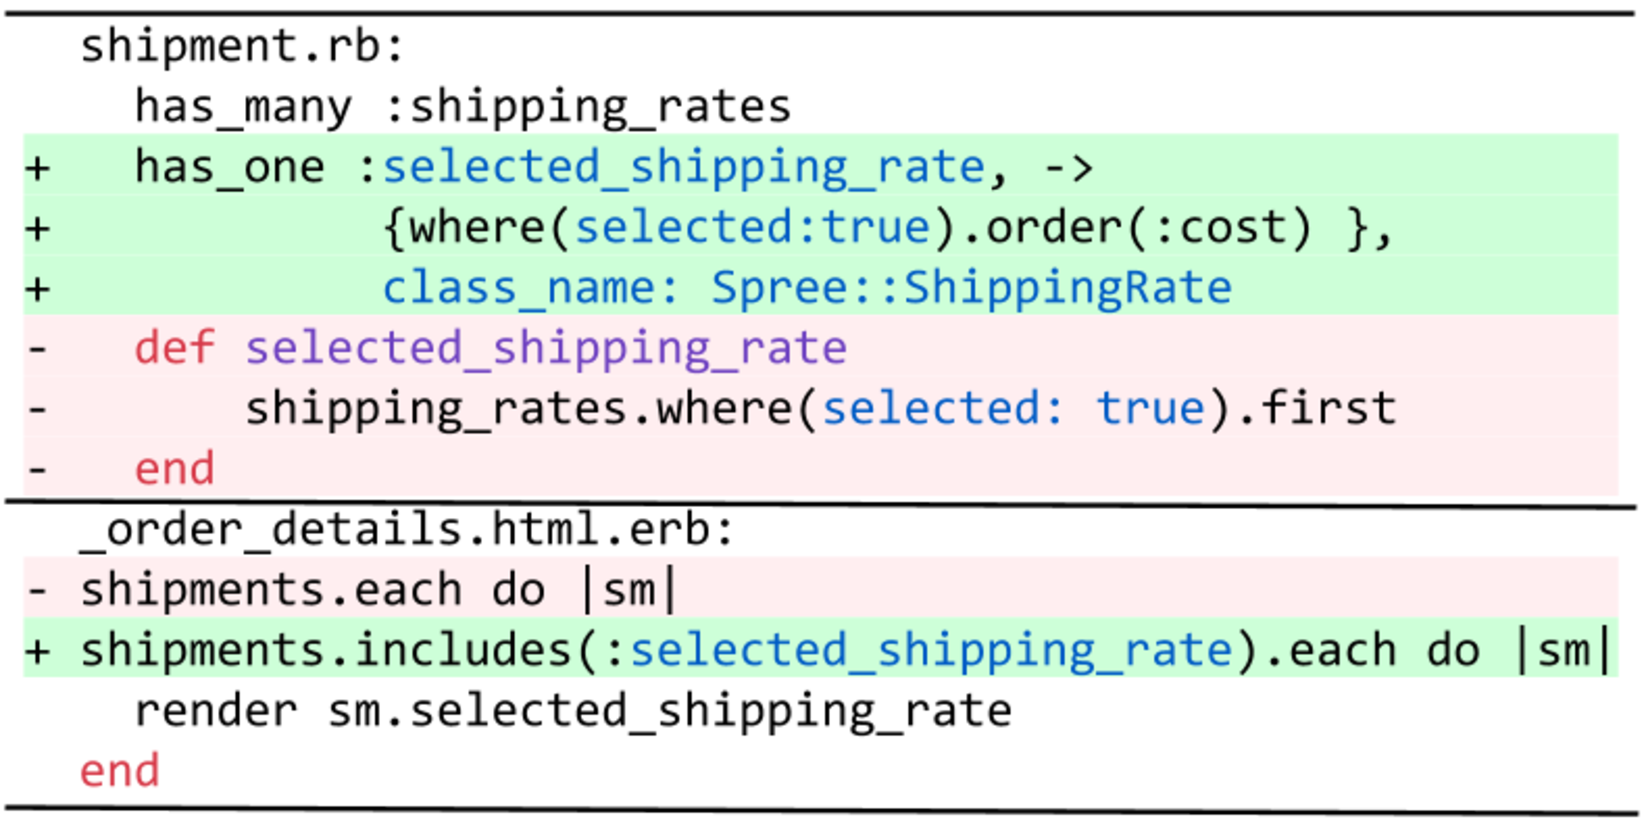
\includegraphics[width=1\columnwidth]{figs/spree7511}
  \caption{Adding association to enable eager loading (Spree)}
  \label{fig:spree7511}
  
\end{figure}
\end{comment}
\vspace{-0.10in}
\subsubsection{Missing Database Indexes (MI)}

Having the appropriate indexes on tables is important for query processing and is a 
well-studied problem \cite{Ullman:1997}. 
As shown in Table \ref{tab:freq}, missing index is the most common performance problem reported in ORM application's bug tracking systems. However, it only appears in three out of the \numpactions problematic actions in latest versions.
We speculate that ORM developers
often do not have the expertise to pick the optimal indexes at the design
phase and hence add table indexes in an incremental way depending on
which query performance becomes a problem after deployment.
%In most of the missing-index issues, an index was added to improve the performance of join queries (7 out of 11), particularly join queries whose \texttt{join} clause contains more than 10 columns (xx out of xx) Missing single and multi-column indexes are both common (about 2:1 ratio)
%.
%missing indexes were so common for several reasons. 
%First, developers of database-backed web applications are often not database optimization experts 
%(partially due to the ORM hiding the database away as an abstraction), and picking the optimal indexes requires understanding the semantics of the application and also how each call to the ORM framework is translated to queries.
%Furthermore, even if developers have the required expertise, they might worry about the cost (in terms of disk and memory space) for creating indexes.
%especially when a table already contains several other indexes. xxx. 
%In fact, xx out of xx missing-index tables in our study were initially released with only one index on its primary key, and only when query performance becomes a problem after deployment will indexes be added in subsequent versions of the application.




\subsection{Application Design Trade-offs}
\label{sec:appdesign}

Developers fix 33 out of the \numissues issue reports by adjusting application display or removing costly functionalities. 
We find similar design problems in latest
versions of 7 out of 12 ORM applications. It is impractical to
completely automate display and functionality design. 
However, our study
shows that ORM developers need tool support, which does not exist yet, to be more informed about the performance implication of their application design decisions.
%found no effectively way to solve the performance problems unless developers throw away some unworthy functionality.
\vspace{-0.10in} 
\subsubsection{Content Display Trade-offs (DT)}
In our study, the most common cause for scalability problems is that a controller action displays \textit{all} database records satisfying certain condition in one page. When the database size increases, the corresponding page takes a lot of time to load due to the increasing amount of data to retrieve and render. This problem contributes to 15 out of the
34 problematic actions that do not scale well in our study. It also appears in 7 out of \numissues issue reports, and is \textit{always} fixed by pagination, i.e., display only a fixed number of records in one page and allow users to navigate to remaining records. 

%As an example, the \texttt{products/index} page in \texttt{Ror\_ecommerce} renders all \textit{products} that are stored in the database. As the number of products increases, the time taken to render the page will increase as well. In practice, users often do not need to see all contents within one page. (e.g., they may only want to see the most popular products). By rendering products by pagination (showing only \alvin{XXX} per page), we find that performance can be improved by $5\times$.

\textcolor{black}{ For example, in \texttt{Diaspora-5335} %named ``\texttt{Paginate cont-}\texttt{acts}'', 
developers used the \texttt{will\_paginate} library~\cite{gem:paginate} to render 25 contacts per page and allow users to see the remaining contacts by clicking the navigation bar at the bottom of the page, instead of showing all contacts within one page as in the old version.
%\texttt{Redmine}, on the other hand, solves a similar problem in 
%\texttt{Redmine-5286} by letting users specify how many issues they want to see within one page.
Clearly, good UI designs can both enhance user experience and improve application performance.} 

%Pagination 
%is widely used in webpage displaying; there are also Rails library support for implementing pagination \cite{gem:paginate}. 
Unfortunately, the lack of pagination still widely exists in latest versions
of ORM applications in our study. This indicates that ORM developers need 
database-aware performance-estimation 
support to remind them of the need to use pagination in webpage design.
\vspace{-0.08in}

\subsubsection{Application Functionality Trade-offs (FT)}
\label{sec:simplifyfeatures}
%When designing the application, without knowing the real workload, it's hard for designers to know the exact time consumed on certain functional feature. As a result, the application may contain some features that cause severe performance problems without bringing much functionality appealing.
%This is particularly a problem in ORM applications, because it is often difficult for developers to know whether and what queries are issued underlying Ruby code, not to mention estimating the query cost.

It is often difficult for ORM developers to estimate performance of a new application feature given that they need to know what queries will be issued by the ORM, how long these queries will execute, and how much data will be returned from the database. In our study, all but two applications have performance issues fixed by developers through removing functionality. 

For example, \texttt{Tracks-870} made a trade-off between performance and functionality by removing a sidebar on the resulting page. This side bar retrieves and displays all the projects and contexts of the current user, and costs a lot of time for users who have participated in many projects.
In the side-bar code, the only data-related part is simply a \texttt{@sidebar.active\_projects} expression, which seems like a trivial
heap access but actually issues a \texttt{SELECT} query and retrieves a lot of data from the database.

As another example, our profiling finds that the \texttt{story.edit} action in the latest version of Lobsters takes 1.5 seconds just to execute one query that determines whether to show the \texttt{guidelines} for users when they edit stories, while the entire page takes 2 seconds to load altogether. Since the  \texttt{guidelines} object only takes very small amount of space to show on the resulting page, removing such checking has negligible impact to the application functionality, yet it would speed up the loading time of that page a lot. 


%\texttt{sidebar} to show the \texttt{actions} and \texttt{contexts} and finally decide the remove \texttt{sidebar}.

In general, performance estimation for applications built using ORMs is important yet has not been done before. It is more difficult as compared to traditional applications due to multiple layers of abstraction. 
We believe combining static analysis with query scalability estimation \cite{armbrust:sigmod13:scale, fan:pods2014:scale} will help developers estimate application performance, as we will discuss in Section \ref{sec:dis}. 
%estimate performance and scalability of ORM code snippets. Including that feature in IDE could greatly help developers in their ORM software design. 


\begin{comment}
\subsection{Potential Solutions}


\subsubsection{Ruby Code Optimization}

\textbf{use more efficient API}
\textbf{use eager loading to prefetch the data}
\textbf{partial to template}
\subsubsection{DB optimization}

\textbf{Add index}
\textbf{Table denormalization}
\subsubsection{Ruby code re-writing}
\textbf{ Paginating}
\end{comment}

